\chapter{\textit{MACRON}}\label{subsec:macron}



O padrão MACRON (\textit{Multiagent Architecture for Cooperative Retrieval ONline}) apresenta um sistema de aquisição de informações \cite{decker1995macron}. Nesta organização, é elaborado um planejamento único que gera sub-objetivos a serem  alcançados por um grupo de agentes que cooperam entre si.

A cooperação entre agentes implica o gerenciamento de interdependências entre suas tarefas. Ao interagirem, os agentes integram e desenvolvem agrupamentos consistentes de informações de alta qualidade a partir de fontes heterogêneas distribuídas \cite{decker1995macron}.  

Tais agentes compartilham informações um com o outro de modo a saberem (i) quais os planos que eles executam para alcançar seus sub-objetivos, (ii) em qual ordem executam tarefas, e (iii) quando as executam. Além disso, os agentes são livres para desenvolver diferentes planos de coleta de informações, a depender da quantidade de tempo que possuem para produzir uma resposta \cite{decker1995macron}. 


\begin{description}
  \item[Nome do padrão:] MACRON, \textit{Multiagent Architecture for Cooperative Retrieval ONline}.
  
    \item[Referências:]    \citeonline{decker1995macron} e \citeonline{shehory1998architectural}.
    
    \item[Categoria:] \textit{Matrix structure}. Isso se deve ao fato de que este padrão possui uma partição bidimensional para unidades: unidades funcionais e unidades de resposta de consulta, a serem descritas a seguir.
    
    \item[Problema:] ocorre quando um informação não pode ser simplesmente recuperada, mas adquirida através de um processo dinâmico, incremental e limitado pelos recursos disponíveis \cite{decker1995macron}.

    \item[Solução:] 

    O padrão MACRON possui os seguintes objetivos: (i) explorar interdependências entre problemas, (ii) gerenciar a incerteza inerente à busca, (iii) compensar inteligentemente a qualidade da solução devido às limitações de recursos, e (iv) explorar ou evitar redundância, conforme necessário \cite{decker1995macron}. 
   
    De acordo com \citeonline{shehory1998architectural}, o sistema consiste nos seguintes agentes ou grupo de agentes:

\begin{itemize}
    \item \textit{\textbf{Query-Manager}} (QM) ou gerente de consulta: recebe uma consulta de um usuário, desenvolve um plano inicial de levantamento de informações de alto nível, recruta agentes das \textit{Functional Units} (FUs) necessárias através dos \textit{Functional Managers} (FMs) para formar uma \textit{Query-Answering Unit} (QAU) e monitora a execução do plano;
    \item \textit{\textbf{Functional Unit}} (FU) ou unidade funcional: uma coleção de agentes que têm acesso a um determinado tipo de recursos de informação. Cada unidade funcional possui um \textit{Functional Manager};
    \item \textbf{\textit{Functional Manager}} (FM) ou gerente funcional: a pedido de um \textit{Query Answering Agent}, o agente  FM atribui tarefas a agentes dentro de sua FU. Embora seja para o mesmo tipo de fontes de informação, os agentes dentro de um FU específica podem ter diferentes conhecimentos. O FM leva essas diferenças em conta ao planejar a tarefa a ser atribuída;
    \item \textit{\textbf{Functional Agent}} (FA) ou agente funcional: planeja a recuperação de informações, solicita-as e as manipula;
    \item \textit{\textbf{Low Level Information Agents}} (LLIA) ou agentes de informação de baixo nível: são simples agentes, cada um especializado em um tipo específico de informações de recuperação. Tal agente recupera as informações solicitadas por um FA, e
    \item \textit{\textbf{Organization Chart Manager}} (OCM) ou gerenciador gráfico da organização: é uma memória organizacional onde os agentes podem procurar informações sobre a disponibilidade e as capacidades de outros agentes. Novos agentes são adicionados ao OCM quando eles se juntam ao sistema dinamicamente, durante o tempo de execução. QMs, FMs e agentes funcionais todos consultam o OCM para localizar os agentes apropriados aos quais eles têm que delegar tarefas. %Note que, embora suporte mudanças dinâmicas na comunidade de agentes, o OCM é um mecanismo centralizado e um único ponto de falha.
\end{itemize}
    
    Na Figura \ref{fig:macron2}, são apresentados os componentes do MACRON e as relações entre eles. Alguns detalhes foram omitidos pelo autor, como a comunicação bidirecional de agentes FA com o OCM e de agentes FM com agentes FAs em sua unidade funcional. Cabe ressaltar que uma vez que o QAU foi formado, o monitoramento das FAs é feito pelo QM responsável pela consulta e não pelo FM.
    
    

    \begin{figure}[h!]
    \centering
    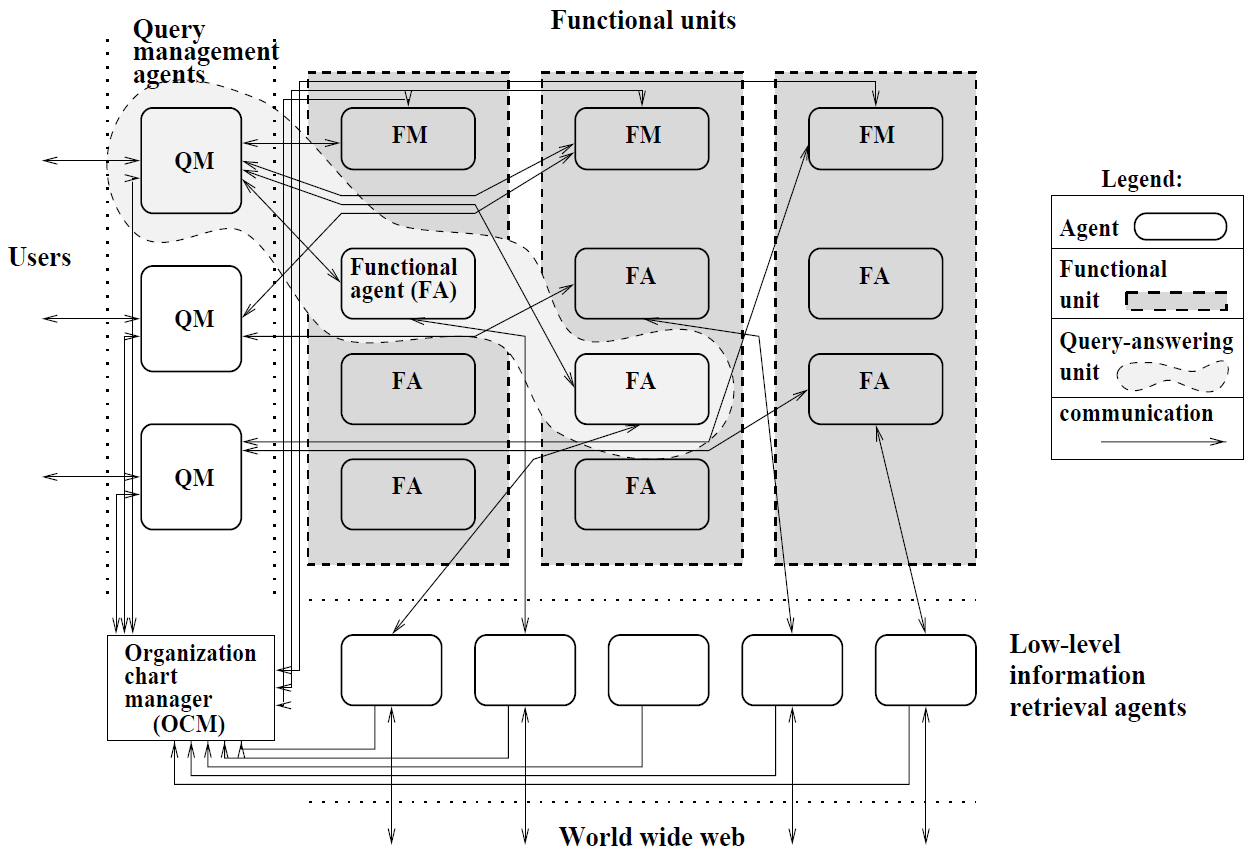
\includegraphics[scale=0.7]{figuras/macron/macron2.png}
    \caption{Organização MACRON. Fonte: \citeonline{shehory1998architectural}.}
    \label{fig:macron2}
\end{figure}
    
Do ponto de vista organizacional, os agentes no MACRON formam uma organização matricial, consistindo em unidades funcionais e de resposta de consulta como apresentado na Figura \ref{fig:macron}. Em uma organização matricial humana, as pessoas pertencem a um grupo funcional de longo prazo e curto prazo. Por exemplo,  em um ambiente de desenvolvimento de software, existe um grupo de \textit{designers} de interface, um grupo de desenvolvedores de software e outro grupo de \textit{designers} de \textit{hardware}, consistindo em grupos de longo prazo. De modo dinâmico, pessoas destes grupos são alocadas para formar um grupo para um projeto de curto prazo. Tais organizações proporcionam flexibilidade ao sistema, em ambientes com mudanças incertas e dinâmicas, permitindo ainda a atribuição e o rastreamento de recursos limitados entre os agentes.

\item[Modelagem:] este padrão pode ser representado pela Figura \ref{fig:macron2}.

\item[Exemplo:] o exemplo a seguir baseia-se em um sistema (Figura \ref{fig:macron}) capaz de recuperar \textit{reviews} de usuários na internet a cerca de um determinado produto.


\begin{figure}[h!]
    \centering
    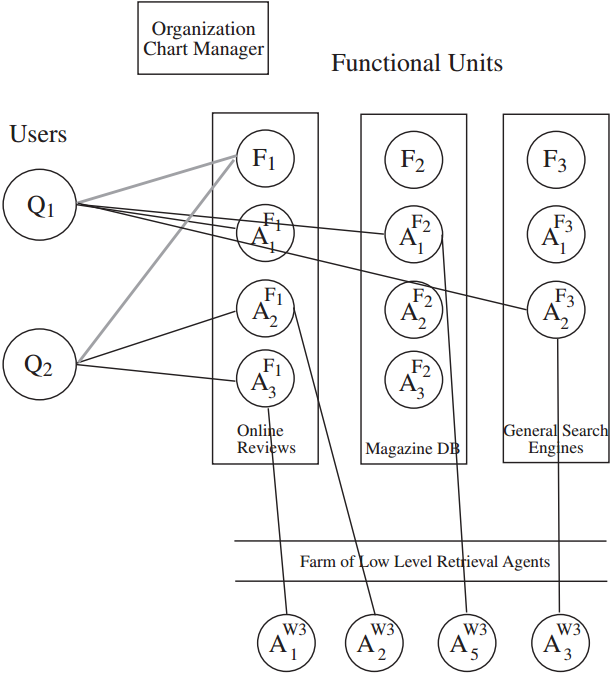
\includegraphics[scale=0.4]{figuras/macron/macron.png}
    \caption{Exemplo de estrutura MACRON. Fonte: \citeonline{decker1995macron}.}
    \label{fig:macron}
\end{figure}

\newpage

Na Figura \ref{fig:macron_example}, o agente QM pode expandir o objetivo inicial \textit{Get Review} para \textit{Get Online Reviews} e \textit{Get Published Reviews}. Ele, então, se comunica com agentes FM para obter \textit{Online Reviews} e \textit{Published Reviews}. Os agentes FM, por sua vez, alocam os objetivos \textit{Get Online Reviews} e \textit{Get Published Reviews} aos agentes das respectivas unidades funcionais (FUs).

\begin{figure}[h!]
    \centering
    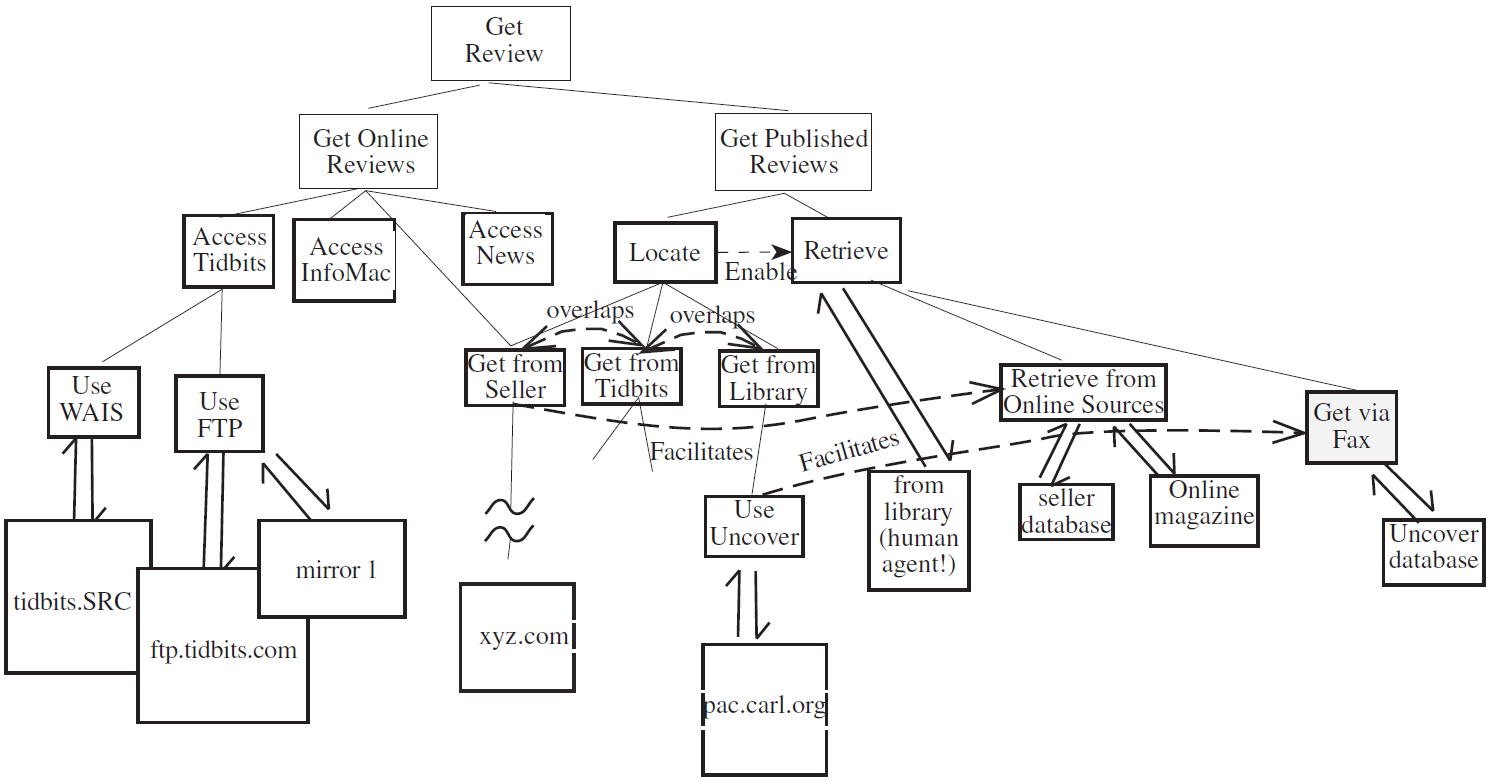
\includegraphics[scale=0.6]{figuras/macron/macron_example.png}
    \caption{Árvore de tarefas para recuperar \textit{reviews} sobre um produto.  Fonte: \citeonline{decker1995macron}.}
    \label{fig:macron_example}
\end{figure}

Suponha-se que cada objetivo é alocado para um agente. Os agentes expandem seus objetivos para alcançar as tarefas primitivas de nível mais baixo, como \textit{Use Wais}, \textit{Use FTP} e \textit{Retrieve Online Magazine}. O agente de consulta verifica o OCM para encontrar o endereço do FM cujas FUs possam obter desempenhar a tarefa \textit{Get Online Reviews}.

Para melhor compreensão da utilidade da estrutura MACRON, a seguir ela será comparada, brevemente, à duas abordagens alternativas. Em uma abordagem de organização de \textbf{agentes com funções fixas}, teríamos equipes de agentes, cada equipe consistindo de pelo menos um membro de cada FU. Essas equipes fixas causam vários problemas: como todas as consultas não precisarão de todos os recursos funcionais, alguns membros da equipe ficarão ociosos. Por outro lado, se um membro da equipe necessário estiver temporariamente indisponível, uma consulta poderá falhar. Em terceiro lugar, à medida que forem introduzidos componentes de aprendizagem nos agentes, as equipes começam a diferenciar e desenvolver diferentes especializações em cada uma de suas áreas funcionais. Se o ambiente é dinâmico, pode-se esperar que surjam novas consultas que seriam mais bem respondidas por combinações de agentes experientes que diferem das equipes fixas oferecidas.

Uma segunda abordagem para se comparar com a estrutura MACRON, seria o outro extremo da abordagem anterior, com uma variedade de \textbf{agentes sem funções fixas}, onde um agente de consultas pode reunir uma equipe de agentes para lidar com uma consulta específica. Neste caso, não há recursos desperdiçados, e não há problemas se um único agente estiver temporariamente indisponível. Este sistema é mais flexível do que a organização funcional fixa.

No entanto, essa abordagem falha em fornecer métodos simples para reunir a melhor equipe possível, especialmente em um sistema cooperativo. São duas importantes perguntas que o agente responsável pelas consultas deve responder: 

\begin{itemize}
    \item Qual dos agentes que anunciam um serviço ele deve realmente entrar em contato e utilizar seu serviço?
    \item À medida que os agentes aprendem e se diferenciam, como eles podem comparar suas habilidades relativas sem se conhecerem?
\end{itemize}

Na organização MACRON, a escolha de um agente funcional é de responsabilidade exclusiva dos gerentes funcionais; que atuam como facilitadores especializados e inteligentes. O MACRON permite o melhor das duas abordagens anteriores: a flexibilidade de montar uma equipe eficiente e a capacidade de atribuir e rastrear de forma inteligente e dinâmica esses recursos do agente.

\item[Implementação:] a fim de demonstrar o padrão MACRON, é utilizado o contexto do exemplo acima. Todos os detalhes da implementação, configuração de ambiente e passos para execução são descritos no Apêndice \ref{appendix:macron}.

\end{description}









